\documentclass[journal,12pt,twocolumn]{IEEEtran}
\usepackage{amsthm}
\allowbreak
\usepackage{setspace}
\usepackage{gensymb}
\singlespacing
\usepackage[cmex10]{amsmath}
\usepackage{caption}
\usepackage{amsthm}

\DeclareUnicodeCharacter{2212}{-}
\usepackage{tikz}
\usepackage{pgfplots}

\usepackage{mathrsfs}
\usepackage{txfonts}
\usepackage{stfloats}
\usepackage{bm}
\usepackage{cite}
\usepackage{cases}
\usepackage{subfig}

\usepackage{longtable}
\usepackage{multirow}

\usepackage{enumitem}
\usepackage{mathtools}
\usepackage{steinmetz}
\usepackage{tikz}
\usepackage{circuitikz}
\usepackage{verbatim}
\usepackage{tfrupee}
\usepackage[breaklinks=true]{hyperref}
\usepackage{graphicx}
\usepackage{tkz-euclide}
\graphicspath{ {./images/} }
\usetikzlibrary{calc,math}
\usepackage{listings}
    \usepackage{color}                                            %%
    \usepackage{array}                                            %%
    \usepackage{longtable}                                        %%
    \usepackage{calc}                                             %%
    \usepackage{multirow}                                         %%
    \usepackage{hhline}                                           %%
    \usepackage{ifthen}                                           %%
    \usepackage{lscape}     
\usepackage{multicol}
\usepackage{chngcntr}

\DeclareMathOperator*{\Res}{Res}

\newcommand{\comb}[2]{{}^{#1}\mathrm{C}_{#2}}

\renewcommand\thesection{\arabic{section}}
\renewcommand\thesubsection{\thesection.\arabic{subsection}}
\renewcommand\thesubsubsection{\thesubsection.\arabic{subsubsection}}

\renewcommand\thesectiondis{\arabic{section}}
\renewcommand\thesubsectiondis{\thesectiondis.\arabic{subsection}}
\renewcommand\thesubsubsectiondis{\thesubsectiondis.\arabic{subsubsection}}


\hyphenation{op-tical net-works semi-conduc-tor}
\def\inputGnumericTable{}                                 %%

\lstset{
%language=C,
frame=single, 
breaklines=true,
columns=fullflexible
}
\begin{document}


\newtheorem{theorem}{Theorem}[section]
\newtheorem{problem}{Problem}
\newtheorem{proposition}{Proposition}[section]
\newtheorem{lemma}{Lemma}[section]
\newtheorem{corollary}[theorem]{Corollary}
\newtheorem{example}{Example}[section]
\newtheorem{definition}[problem]{Definition}

\newcommand{\BEQA}{\begin{eqnarray}}
\newcommand{\EEQA}{\end{eqnarray}}
\newcommand{\define}{\stackrel{\triangle}{=}}
\bibliographystyle{IEEEtran}
\raggedbottom
\setlength{\parindent}{0pt}
\providecommand{\mbf}{\mathbf}
\providecommand{\pr}[1]{\ensuremath{\Pr\left(#1\right)}}
\providecommand{\qfunc}[1]{\ensuremath{Q\left(#1\right)}}
\providecommand{\sbrak}[1]{\ensuremath{{}\left[#1\right]}}
\providecommand{\lsbrak}[1]{\ensuremath{{}\left[#1\right.}}
\providecommand{\rsbrak}[1]{\ensuremath{{}\left.#1\right]}}
\providecommand{\brak}[1]{\ensuremath{\left(#1\right)}}
\providecommand{\lbrak}[1]{\ensuremath{\left(#1\right.}}
\providecommand{\rbrak}[1]{\ensuremath{\left.#1\right)}}
\providecommand{\cbrak}[1]{\ensuremath{\left\{#1\right\}}}
\providecommand{\lcbrak}[1]{\ensuremath{\left\{#1\right.}}
\providecommand{\rcbrak}[1]{\ensuremath{\left.#1\right\}}}
\theoremstyle{remark}
\newtheorem{rem}{Remark}
\newcommand{\sgn}{\mathop{\mathrm{sgn}}}
\providecommand{\abs}[1]{$\left\vert#1\right\vert$}
\providecommand{\res}[1]{\Res\displaylimits_{#1}} 
\providecommand{\norm}[1]{$\left\lVert#1\right\rVert$}
%\providecommand{\norm}[1]{\lVert#1\rVert}
\providecommand{\mtx}[1]{\mathbf{#1}}
\providecommand{\mean}[1]{E$\left[ #1 \right]$}
\providecommand{\fourier}{\overset{\mathcal{F}}{ \rightleftharpoons}}
%\providecommand{\hilbert}{\overset{\mathcal{H}}{ \rightleftharpoons}}
\providecommand{\system}{\overset{\mathcal{H}}{ \longleftrightarrow}}
	%\newcommand{\solution}[2]{\textbf{Solution:}{#1}}
\newcommand{\solution}{\noindent \textbf{Solution: }}
\newcommand{\cosec}{\,\text{cosec}\,}
\providecommand{\dec}[2]{\ensuremath{\overset{#1}{\underset{#2}{\gtrless}}}}
\newcommand{\myvec}[1]{\ensuremath{\begin{pmatrix}#1\end{pmatrix}}}
\newcommand{\mydet}[1]{\ensuremath{\begin{vmatrix}#1\end{vmatrix}}}
\numberwithin{equation}{subsection}
\makeatletter
\@addtoreset{figure}{problem}
\makeatother
\let\StandardTheFigure\thefigure
\let\vec\mathbf
\renewcommand{\thefigure}{\theproblem}
\def\putbox#1#2#3{\makebox[0in][l]{\makebox[#1][l]{}\raisebox{\baselineskip}[0in][0in]{\raisebox{#2}[0in][0in]{#3}}}}
     \def\rightbox#1{\makebox[0in][r]{#1}}
     \def\centbox#1{\makebox[0in]{#1}}
     \def\topbox#1{\raisebox{-\baselineskip}[0in][0in]{#1}}
     \def\midbox#1{\raisebox{-0.5\baselineskip}[0in][0in]{#1}}
\vspace{3cm}
\title{Assignment 3}
\author{Vijay Varma - AI20BTECH11012}
\maketitle
\newpage
\bigskip
\renewcommand{\thefigure}{\theenumi}
\renewcommand{\thetable}{\theenumi}


Download all python codes from 
\begin{lstlisting}
https://github.com/KBVijayVarma/AI1103-Assignment-3
\end{lstlisting}
%
Download latex-tikz codes from 
%
\begin{lstlisting}
https://github.com/KBVijayVarma/AI1103-Assignment-3
\end{lstlisting}
\section*{\textbf{Problem GATE 2015 (MA), Q. 8}}
Let $X \sim B(5,\frac{1}{2})$ and $Y \sim U(0,1)$. Then $\frac{P(X + Y \leq 2)}{P(X + Y \geq 5)}$ is equal to 

(where 

$B(n,p)$ : Binomial distribution with n trials and success probability p; $n \in \{1,2, \dots \}$ and  $p \in (0,1)$

U(a,b) : Uniform distribution on the interval $(a,b), -\infty < a < b < \infty$  )
\section*{\textbf{Solution}}
Given X is a Binomial Random Variable with 5 trails and success probability $p=0.5$ and Y is a Continuous Random Variable over the interval $(0,1)$.

So, $X \in \{0,1,2,3,4,5\}$ and $Y = U(0,1)$

Since X and Y are Independent Random Variables,
\begin{align}
\pr{X + Y \leq 2} &= \pr{X = a, Y \leq 2-a} \\
&= \sum_{a = 0}^{a = 2} \pr{X = a}\pr{Y \leq 2-a} 
\end{align}
\begin{multline}
\pr{X + Y \leq 2} = \pr{X = 0}\pr{Y \leq 2} \label{0.0.3} \\ 
+ \pr{X = 1}\pr{Y \leq 1} + \pr{X = 2}\pr{Y \leq 0}    
\end{multline}

Since $X$ is a Binomial Random Variable,
\begin{align}
\pr{X = k} = \begin{cases}
\comb{n}{k}p^{n-k}(1-p)^{k} & 0 \leq k \leq 5 \\
0 & otherwise
\end{cases} \label{0.0.4}
\end{align}
Substituting the values of n = 5 and p = $\frac{1}{2}$ in \eqref{0.0.4}, we get
\begin{align*}
\pr{X = k} = \comb{5}{k} \left(\frac{1}{2} \right)^{5-k} \left(\frac{1}{2} \right)^{k} = \comb{5}{k} \left(\frac{1}{2} \right)^{5}    
\end{align*}
Also, the Cumulative Distribution Function of $Y$ is
defined as
\begin{align}
CDF(Y) = F_Y(a) = \pr{Y \leq a} = \begin{cases}
0 & a \leq 0 \\
a & 0 < a < 1 \\ 
1 & a \geq 1
\end{cases} \label{0.0.5}   
\end{align}
By substituting the probability values from \eqref{0.0.4} and \eqref{0.0.5} in \eqref{0.0.3}, we get
\begin{multline}
\pr{X + Y \leq 2} = \comb{5}{0} \left(\frac{1}{2} \right)^{5}(1) + \comb{5}{1} \left(\frac{1}{2} \right)^{5}(1) \\ + \comb{5}{2} \left(\frac{1}{2} \right)^{5}(0)    
\end{multline}
\begin{align}
&= (1)\left(\frac{1}{32} \right) + (5)\left(\frac{1}{32} \right) + 0 \\
&= \left(\frac{1}{32} \right) + \left(\frac{5}{32} \right) \\
&= \frac{6}{32} \\
\pr{X + Y \leq 2} &= \frac{3}{16}    
\end{align}
Now,
\begin{align}
\pr{X + Y \geq 5} &= 1 - \pr{X + Y <  5}
\end{align}
\begin{multline}
= 1 - [\pr{X + Y \leq 5} - \\ \pr{X + Y = 5}] \label{0.0.12}    
\end{multline}
But, as Y is a Continuous Random Variable over $(0,1)$, so $\pr{Y = k } = 0$  $\forall$ k $\in [0,1]$ . Therefore considering all possible cases,
\begin{multline}
\pr{X + Y = 5} = \pr{X = 4}\pr{Y = 1} \\ + \pr{X = 5}\pr{Y = 0}    
\end{multline}
\begin{align}
&= \pr{X = 4}(0) + \pr{X = 5}(0) \\
&= 0 + 0 
\end{align}
\begin{align}
\pr{X + Y = 5} &= 0 \label{0.0.16}    
\end{align}
Hence, by substituting \eqref{0.0.16} in \eqref{0.0.12}, we get
\begin{align}
\pr{X + Y \geq 5} &= 1 - [\pr{X + Y \leq 5} -  0] \\
\pr{X + Y \geq 5} &= 1 - \pr{X + Y \leq 5} \\
\pr{X + Y \geq 5} &= 1 - \pr{X = a, Y \leq 5 - a}
\end{align}
\begin{align}
&= 1 - \left[\sum_{a = 0}^{a = 5} \pr{X = a}\pr{Y \leq 5-a} \right]     
\end{align}
\begin{multline}
= 1 - [ \pr{X = 0}\pr{Y \leq 5} + \pr{X = 1}\pr{Y \leq 4} \\
+ \pr{X = 2}\pr{Y \leq 3} + \pr{X = 3}\pr{Y \leq 2} \\
+ \pr{X = 4}\pr{Y \leq 1} + \pr{X = 5}\pr{Y \leq 0} ] \label{0.0.21}    
\end{multline}


By substituting the probability values from \eqref{0.0.4} and \eqref{0.0.5} in \eqref{0.0.21}, we get
\begin{multline}
\pr{X + Y \geq 5} = 1 - [\comb{5}{0}\left(\frac{1}{2}\right)^{5}(1) + \comb{5}{1}\left(\frac{1}{2}\right)^{5}(1) + \\ \comb{5}{2}\left(\frac{1}{2}\right)^{5}(1) + 
\comb{5}{3}\left(\frac{1}{2}\right)^{5}(1) + \\
\comb{5}{4}\left(\frac{1}{2}\right)^{5}(1) + 
\comb{5}{5}\left(\frac{1}{2}\right)^{5}(0)]  
\end{multline}
\begin{multline}
\pr{X + Y \geq 5} = 1 - \left(\frac{1}{2}\right)^{5} [\comb{5}{0} + \comb{5}{1} \\ + \comb{5}{2} + \comb{5}{3} + \comb{5}{4}]    
\end{multline}
\begin{align}
&= 1 - \left(\frac{1}{32}\right)\left[1 + 5 + 10 + 10 + 5 \right] \\
&= 1- \left(\frac{1}{32}\right)\left[31 \right] = \frac{1}{32}
\end{align}
Hence,
$\pr{X + Y \leq 2} = \frac{3}{16}$ and $\pr{X + Y \geq 5} = \frac{1}{32}$.
\begin{align*}
\therefore \frac{\pr{X + Y \leq 2}}{\pr{X + Y \geq 5}} = \frac{\frac{3}{16}}{\frac{1}{32}} = 6. \\
\therefore \frac{\pr{X + Y \leq 2}}{\pr{X + Y \geq 5}} = 6    
\end{align*}
Hence, the required ratio is 6 .

\begin{figure}[h]
    \centering
    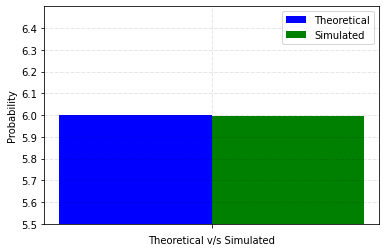
\includegraphics[width = \columnwidth]{Figure_1.png}
    \caption{}
    \label{fig:my_label}
\end{figure}

\end{document}